
%(BEGIN_QUESTION)
% Copyright 2013, Tony R. Kuphaldt, released under the Creative Commons Attribution License (v 1.0)
% This means you may do almost anything with this work of mine, so long as you give me proper credit

Calculate the amount and direction of current through resistor $R_2$ in this opamp circuit, given the output voltage and resistor values shown.  Assume the opamp is capable of ``rail-to-rail'' output voltage swings, and that the output voltage is specified in reference to ground.  Be sure to sketch your current arrow in the direction of {\it conventional} flow:

$$\includegraphics[width=15.5cm]{i01952x01.eps}$$

$I_{R2}$ = 

\underbar{file i01952}
%(END_QUESTION)





%(BEGIN_ANSWER)

$I_{R2}$ = 0.4625 mA (arrow pointing upwards)

%(END_ANSWER)





%(BEGIN_NOTES)

{\bf This question is intended for exams only and not worksheets!}.

%(END_NOTES)

